 

\section{Diseño de la aplicación}

% Diagramas, explicación, etc. M.I.

\subsection{Post}

\begin{figure}[H]
\centering
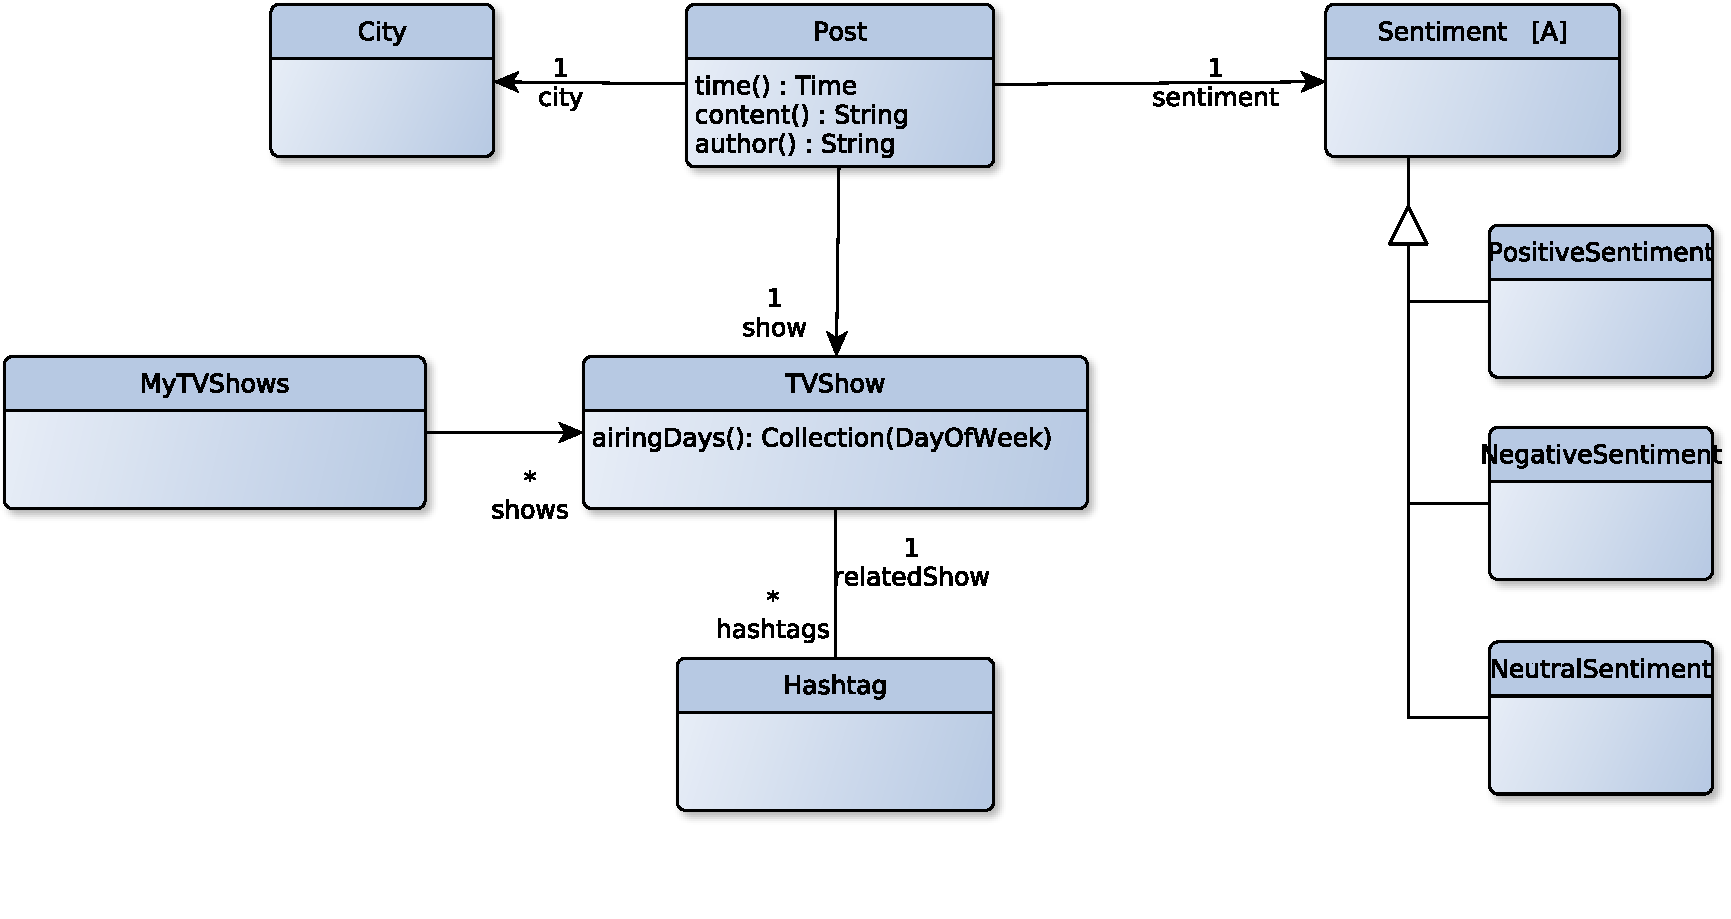
\includegraphics[width=\textwidth]{graph/clase/show.pdf}
\caption{Post}
\end{figure}

El \emph{post} es el elemento básico de esta aplicación, y consiste en un mensaje enviado a través de una red social. En principio es la representación de los datos de un \emph{tweet} que son útiles en nuestro programa, y también puede representar estos mismos datos, obtenidos de una red social distinta de \emph{Twitter}. Contiene algunos datos básicos como autor, texto del mensaje y fecha/hora de envío. También tiene un indicador de la ciudad desde la que se mandó el mensaje, en caso de que el autor haya activado la localización por GPS y de esa forma se pueda identificar su procedencia. Este indicador resulta útil para la vista de popularidad en mapa. Cada post también está vinculado con un único show de TV, el cual se le asigna basándose en palabras claves contenidas en el mensaje. Por último, posee un indicador de sentimiento, que lo clasifica como positivo, negativo o neutro.

\subsection{Post Filterer}

\begin{figure}[H]
\centering
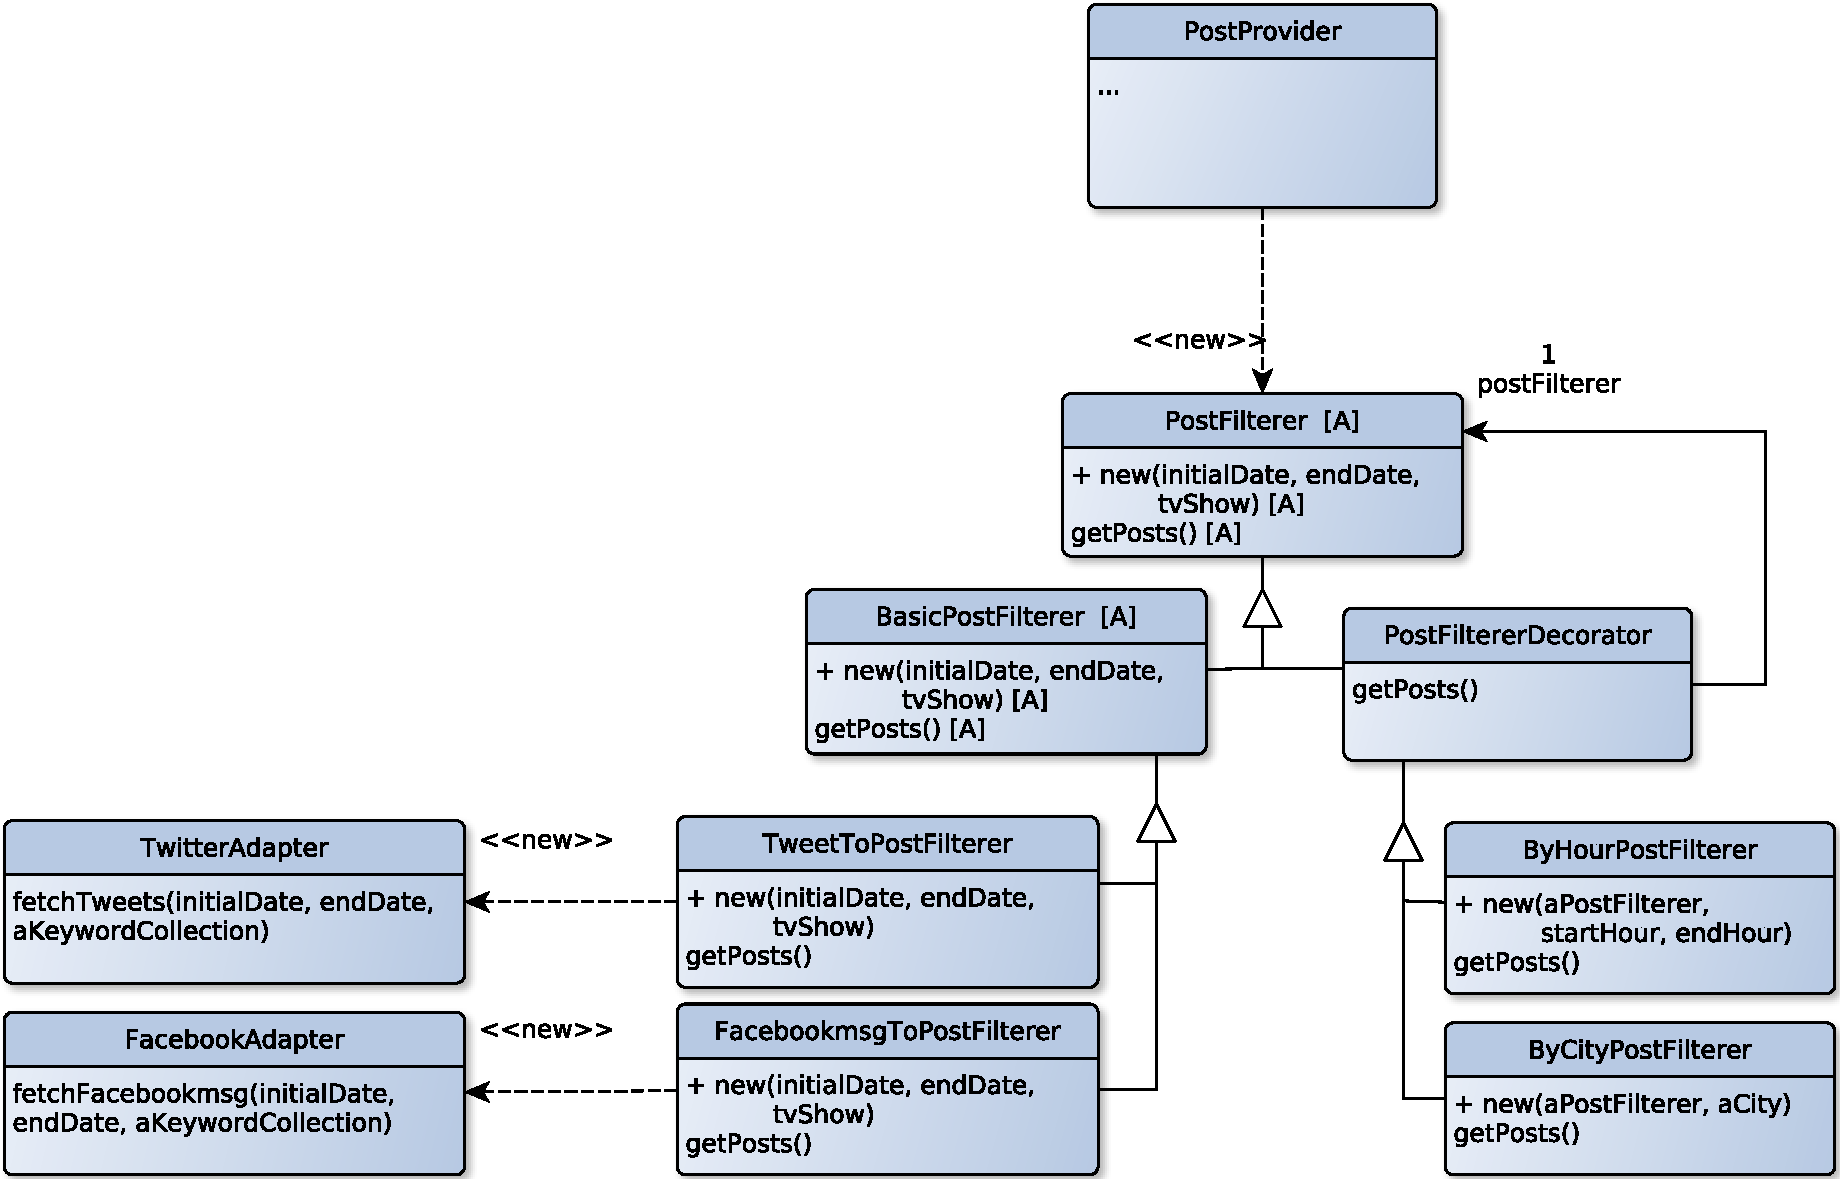
\includegraphics[width=\textwidth]{graph/clase/filterer.pdf}
\caption{Post Filterer}
\end{figure}

\subsection{Sentiment Analyisis}

\begin{figure}[H]
\centering
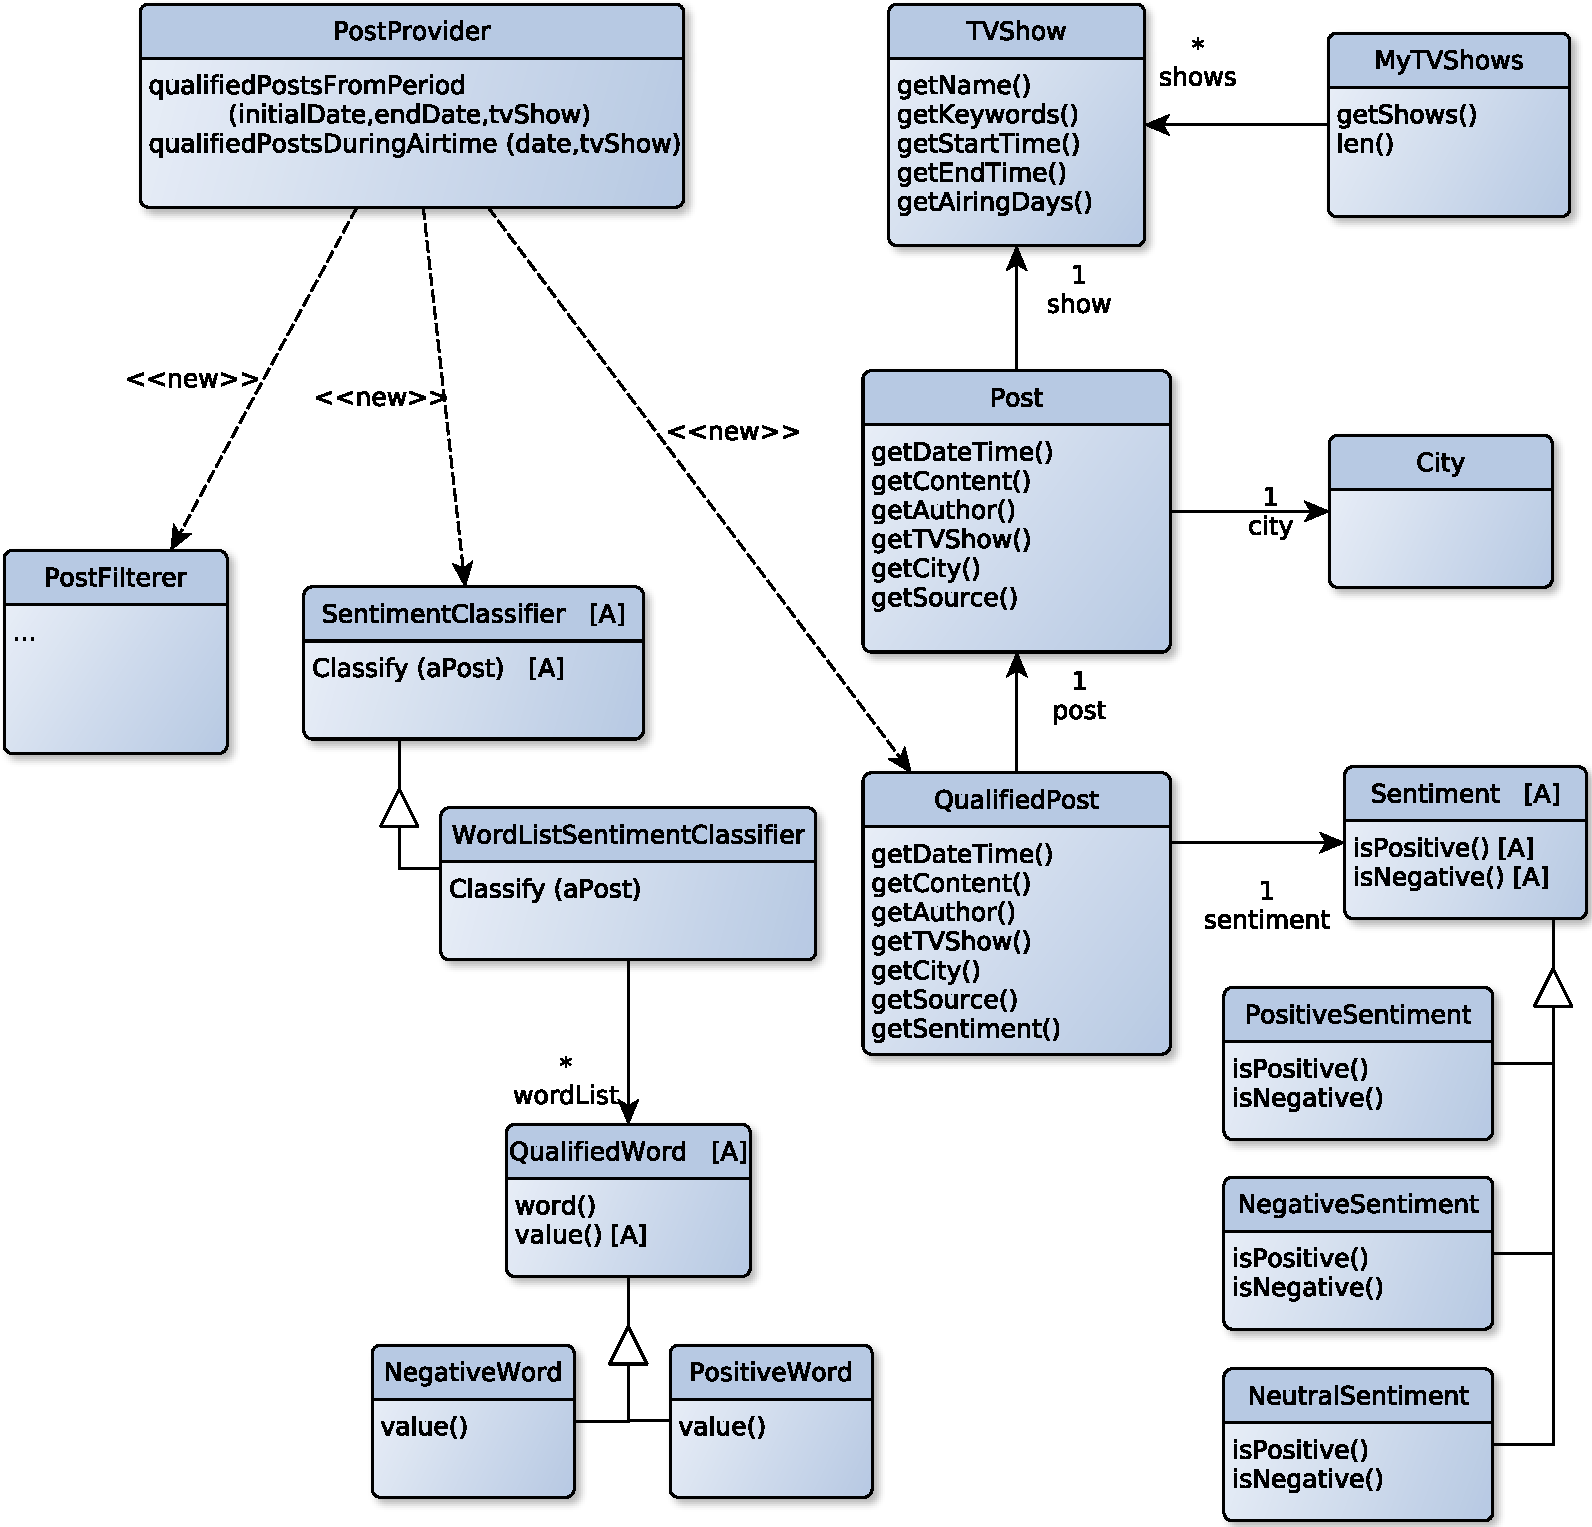
\includegraphics[width=\textwidth]{graph/clase/classifier.pdf}
\caption{Sentiment Classifier}
\end{figure}

Este es un módulo de \emph{Sentiment Analyisis}, que consiste de un clasificador que asigna un valor a cada post y es llamado luego de recibir los datos de la red social e integrarlos al modelo de la aplicación. Existen tres valores para el sentimiento: positivo, negativo y neutro, y la manera de clasificar los posts es transparente al resto de las funcionalidades. En esta primera versión del programa, se usa un clasificador simple que lee de un corpus de palabras puntuadas como positivas o negativas, y realiza la clasificación según la cantidad de palabras de cada tipo que aparecen en cada mensaje. Se espera que a futuro se diseñe un nuevo clasificador con un criterio más complejo, y cuando esté implementado, se sustituya el que existe actualmente.


\subsection{Meters \& Views}

\begin{figure}[H]
\centering
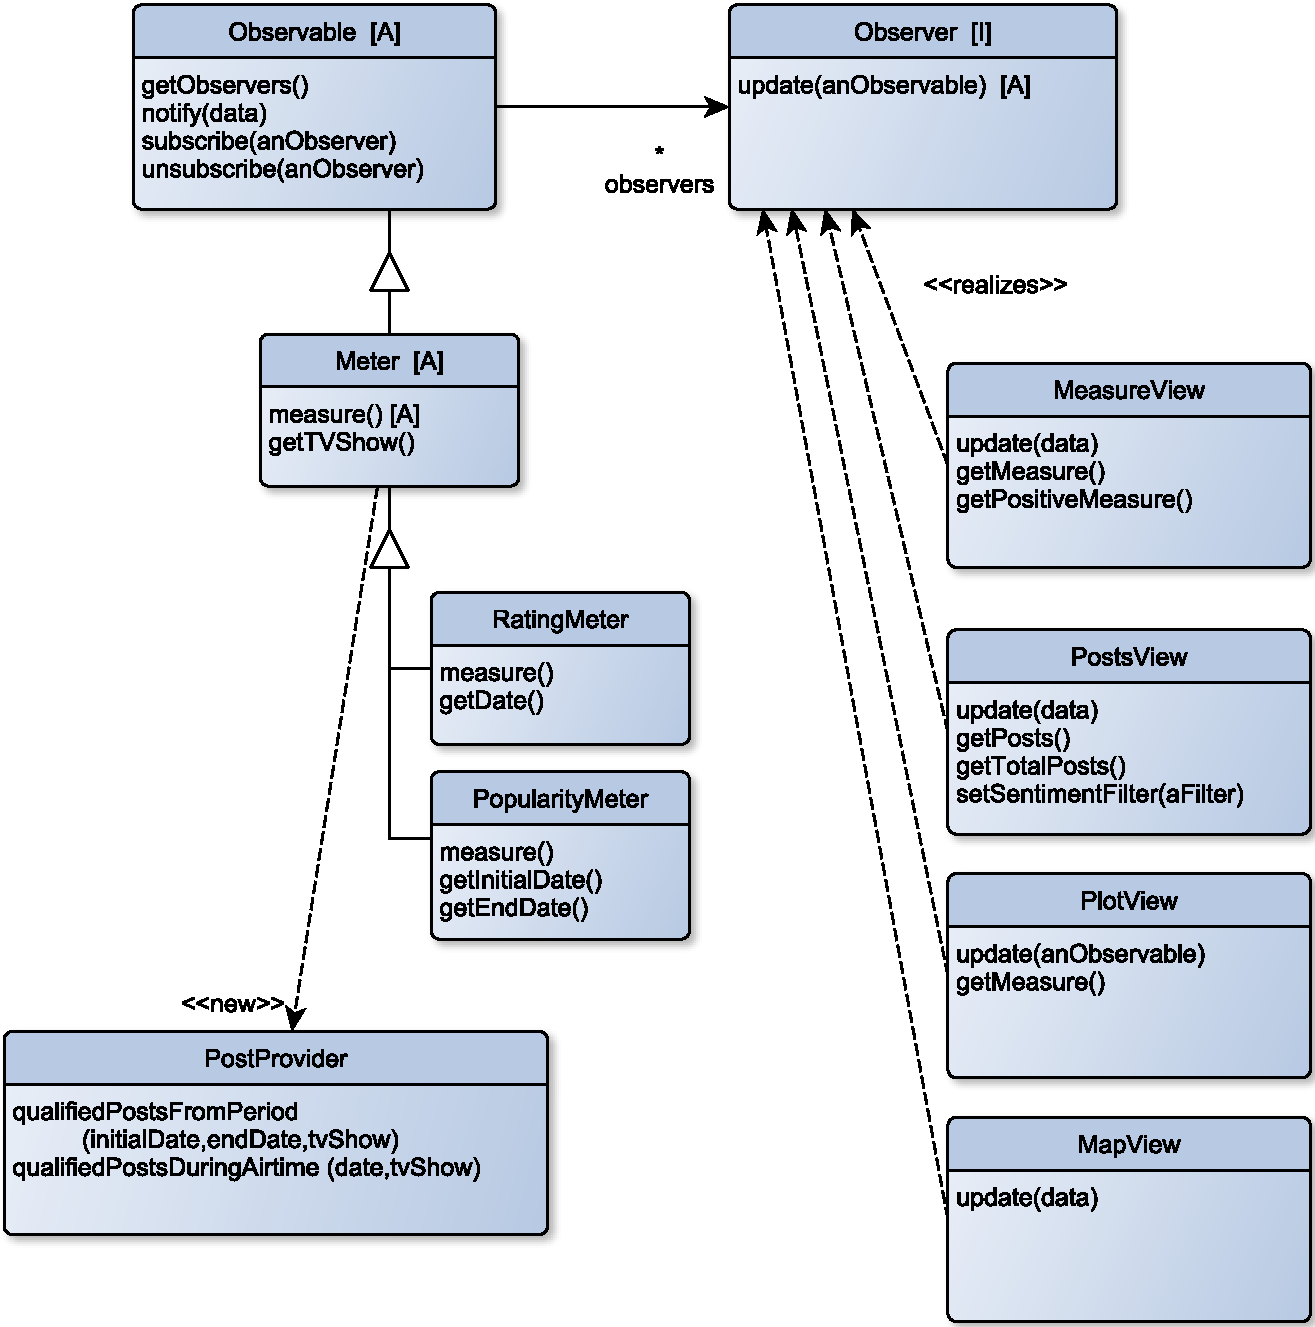
\includegraphics[width=0.8\textwidth]{graph/clase/meters.pdf}
\caption{Meters \& Views}
\end{figure}

Existen dos maneras de realizar mediciones en la aplicación: el rating y la popularidad. El rating consiste en una medición de la cantidad de posts recibidos para un programa en determinada fecha, durante el horario de emisión del programa, con un peso asignado según el sentimiento del mensaje. El rating puede consultarse ``en vivo'' para la fecha actual, mientras un programa se está emitiendo, y en ese caso se actualizará cada 10 segundos la información obtenida. La popularidad es una medición de la cantidad de posts de un programa, dado un intervalo de tiempo, en cualquier horario, también pesados según sentimiento.

En la aplicación hay varias formas de visualizar esta información: la funcionalidad básica es la de mostrar un número que represente la medición de rating o popularidad (que aparece nombrada como MeasureView). Se puede pedir que el resultado se muestre en un gráfico. También hay una funcionalidad para poder leer los mensajes concretos que la aplicación obtuvo y usó para sus cálculos. Estos mensajes se muestran con autor, contenido y fecha, y se los puede filtrar de acuerdo a su sentimiento, en caso de que el usuario quiera ver u ocultar algún tipo de contenido. Por último está la opción de ver los posts en un mapa, donde se los clasifica por área geográfica y se muestra el valor de la medición para cada zona urbana principal.

Cada una de estas vistas es independiente de las demás y trabaja con información que puede obtener del medidor que le corresponde. Esto permite que se puedan agregar o modificar los tipos de vista existentes sin un gran impacto en el resto de la aplicación, y además hace que no sea necesario mantener activas las vistas que el usuario no solicitó.

\subsection{Interfaz de usuario}

La interfaz de usuario es el elemento que coordina y da inicio al nivel más alto de la aplicación. Su responsabilidad es permitir que el usuario active las funcionalidades que desea usar, y eso lleve a crear los objetos necesarios. Cada vez que el usuario seleccione un programa de TV de la lista, y pida ver el rating o la popularidad de dicho programa para un intervalo, se creará un medidor correspondiente a los datos recibidos. De forma similar, cada vez que se seleccione una nueva manera de visualizar los datos, la interfaz pedirá la creación de una vista vinculada al medidor, para que muestre la información.